\chapter{Konzept und Systemdesign}
\printmyminitoc{1}

\section{Aufbau Schiffsysteme}
Wie werden die Motoren im Schiff angesteuert?
Welche Angriffsmöglichkeiten gibt es?
Wie wird das Ruder angesteuert?
Gibt es noch weitere wichtige Systeme?
\begin{itemize}
    \item einzelnen Can-Bus für jeden Gashebel
    \item Serielle Kommunikation bei Autopilot
    \item Autopilot kann nur das Ruder steuern
\end{itemize}

\section{Steuerungslogik des Controllers}
Der benutzte Controller ist ein Xbox Series X Controller. Dieser wurde gewählt, da er eine gute Haptik hat und weit
verbreitet ist. Zusätzlich ist er kabellos und kann somit frei bewegt werden. Um die Steuerung des Schiffes zu
ermöglichen, müssen die Eingaben des Controllers in Steuerbefehle umgewandelt werden. Dies passiert auf dem 
Raspberry Pi. Der Controller wird über Bluetooth mit dem Raspberry Pi verbunden. Dort werden die Eingaben des Controllers
ausgelesen und in einem Python-Programm in Steuerbefehle umgewandelt. \\
Um eine einfache Steuerung zu ermöglichen, wird im folgenden die Tastenbelegung aufgeschlüsselt.
Um alle gewünschten Funktionen umzusetzen, werden nicht alle Tasten benötigt. 

\begin{figure}[H]
    \centering
    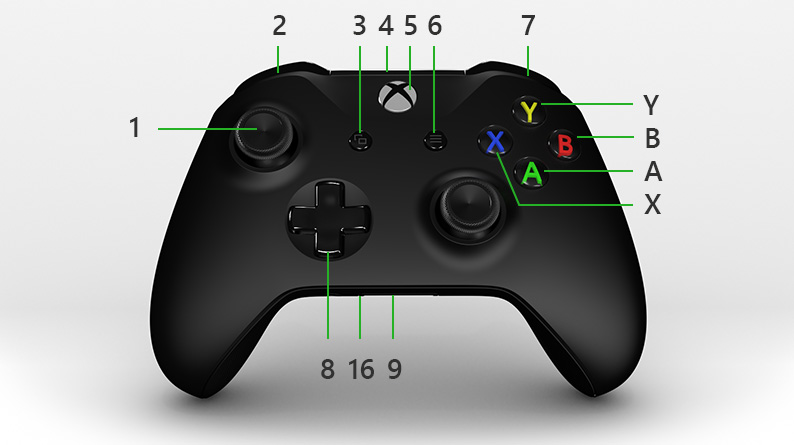
\includegraphics[scale=0.5]{images/vorderseite.jpg}
    \caption{Vorderseite des Controllers \cite{XboxController}(letzter Zugriff: 24.01.2025)}
    \label{fig:vorderseite}
\end{figure}

\begin{figure}[H]
    \centering
    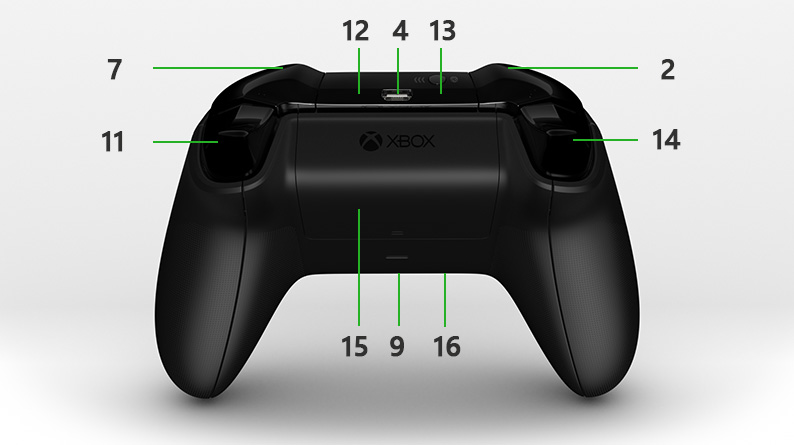
\includegraphics[scale=0.5]{images/rueckseite.jpg}
    \caption{Rückseite des Controllers \cite{XboxController}(letzter Zugriff: 24.01.2025)}
    \label{fig:rueckseite}
\end{figure}

\begin{table}[H]
    \begin{tabular}{|c|c|}
    \hline
    \rowcolor[gray]{0.8}
     Nummerierung der Taste & Funktion \\ \hline 
     1 & Bewegung des Ruders \\ \hline 
     2 & Reduzierung der linken Gashebelposition \\ \hline 
     7 & Reduzierung der rechten Gashebelposition \\ \hline
     11 & Erhöhung der rechten Gashebelposition \\ \hline
     14 & Erhöhung der linken Gashebelposition \\ \hline
     B + 2 & Umschalten des Rückwärtsgangs am linken Motor \\ \hline
     B + 7 & Umschalten des Rückwärtsgangs am rechten Motor \\ \hline
     B + 2 + 7 & Umschalten des Rückwärtsgangs an beiden Motoren \\
      & (basierend auf dem derzeitigen Gang am rechten Motor) \\ \hline
    \end{tabular}
\end{table}
Das Einlegen des Rückwärtsgangs ist durch eine Tastenkombination so gewählt, dass es nicht aus Versehen passieren kann.
Mit jeweils der Taste 2 oder 7 wird die Gashebelposition reduziert. Mit der zusätzlichen Betätigung der Taste B wird der 
Rückwärtsgang eingelegt an dem jeweiligen Motor. Wenn die Tasten 2, 7 und B gleichzeitig betätigt werden, 
wird der Rückwärtsgang für beide Motoren gleichzeitig umgeschalten. Dies ist so gewählt, da eine Verzögerung bei dem
Umschalten eines Rückwärtsgangs von 10 Sekunden eingebaut ist. Das soll dem Getriebe ermöglichen, den Gang zu wechseln
ohne eine direkte Gaseingabe. Nun muss es aber auch möglich sein, beide Rückwärtsgänge gleichzeitig umzuschalten, daher 
die vergleichsweise komplexe Tastenkombination.



\section{Integration des Rogue Device}
Damit der Controller die Steuerbefehle an das Schiff senden kann, muss das Rogue Device in das System integriert werden.
In diesem Fall ist das Rogue Device der Raspberry Pi. Damit dieser möglichst unbemerkt in das System integriert werden könnte,
muss der Controller drahtlos verbunden werden. Um die Kommunikation von dem Rogue Device zu dem Schiff zu ermöglichen, müssen
die einzelnen Systeme angesteuert werden. Um die Gashebelposition zu verändern, wird der Raspberry Pi mit dem Can-Bus des Schiffes
verbunden. 
\begin{itemize}
    \item Stromversorgung des Raspberry Pi (Battery Pack oder Steckdose)
\end{itemize}

Sollte der Gashebel in der normalen Benutzung vom Schiffsführer benutzt werden, wird ein Signal an den Can-Bus gesendet. Dieses Signal wird dann an die Motoren weitergeleitet.
Um diese Eingabe zu verhindern, muss auf diese Nachricht geachtet und reagiert werden. Mit dem Lesen des Can-Bus kann die 
entsprechende Nachricht entdeckt werden. Dann kann eine Nachricht von dem Rogue Device gesendet werden, um die Gashebelposition
zu überschreiben.
\\
Um eine Rückmeldung zu erhalten, wie die gewünschte Gashebel- und Ruderposition ist, sollte mit einer einfachen App
gearbeitet werden. Diese App kann dann die gewünschten Positionen anzeigen. Ein kleiner OLED-Bildschirm könnte auch benutzt 
werden. Allerdings hat dieser den Nachteil, dass er physisch an den Raspberry Pi angeschlossen werden muss. Damit 
ist keine Rückmeldung möglich, wenn dieser als Rogue Device in dem System versteckt angeschlossen ist.
Um die Kommunikation zwischen dem Raspberry Pi und dem Handy mit der App zu ermöglichen, wird Bluetooth benutzt.

\begin{figure}[H]
    \centering
    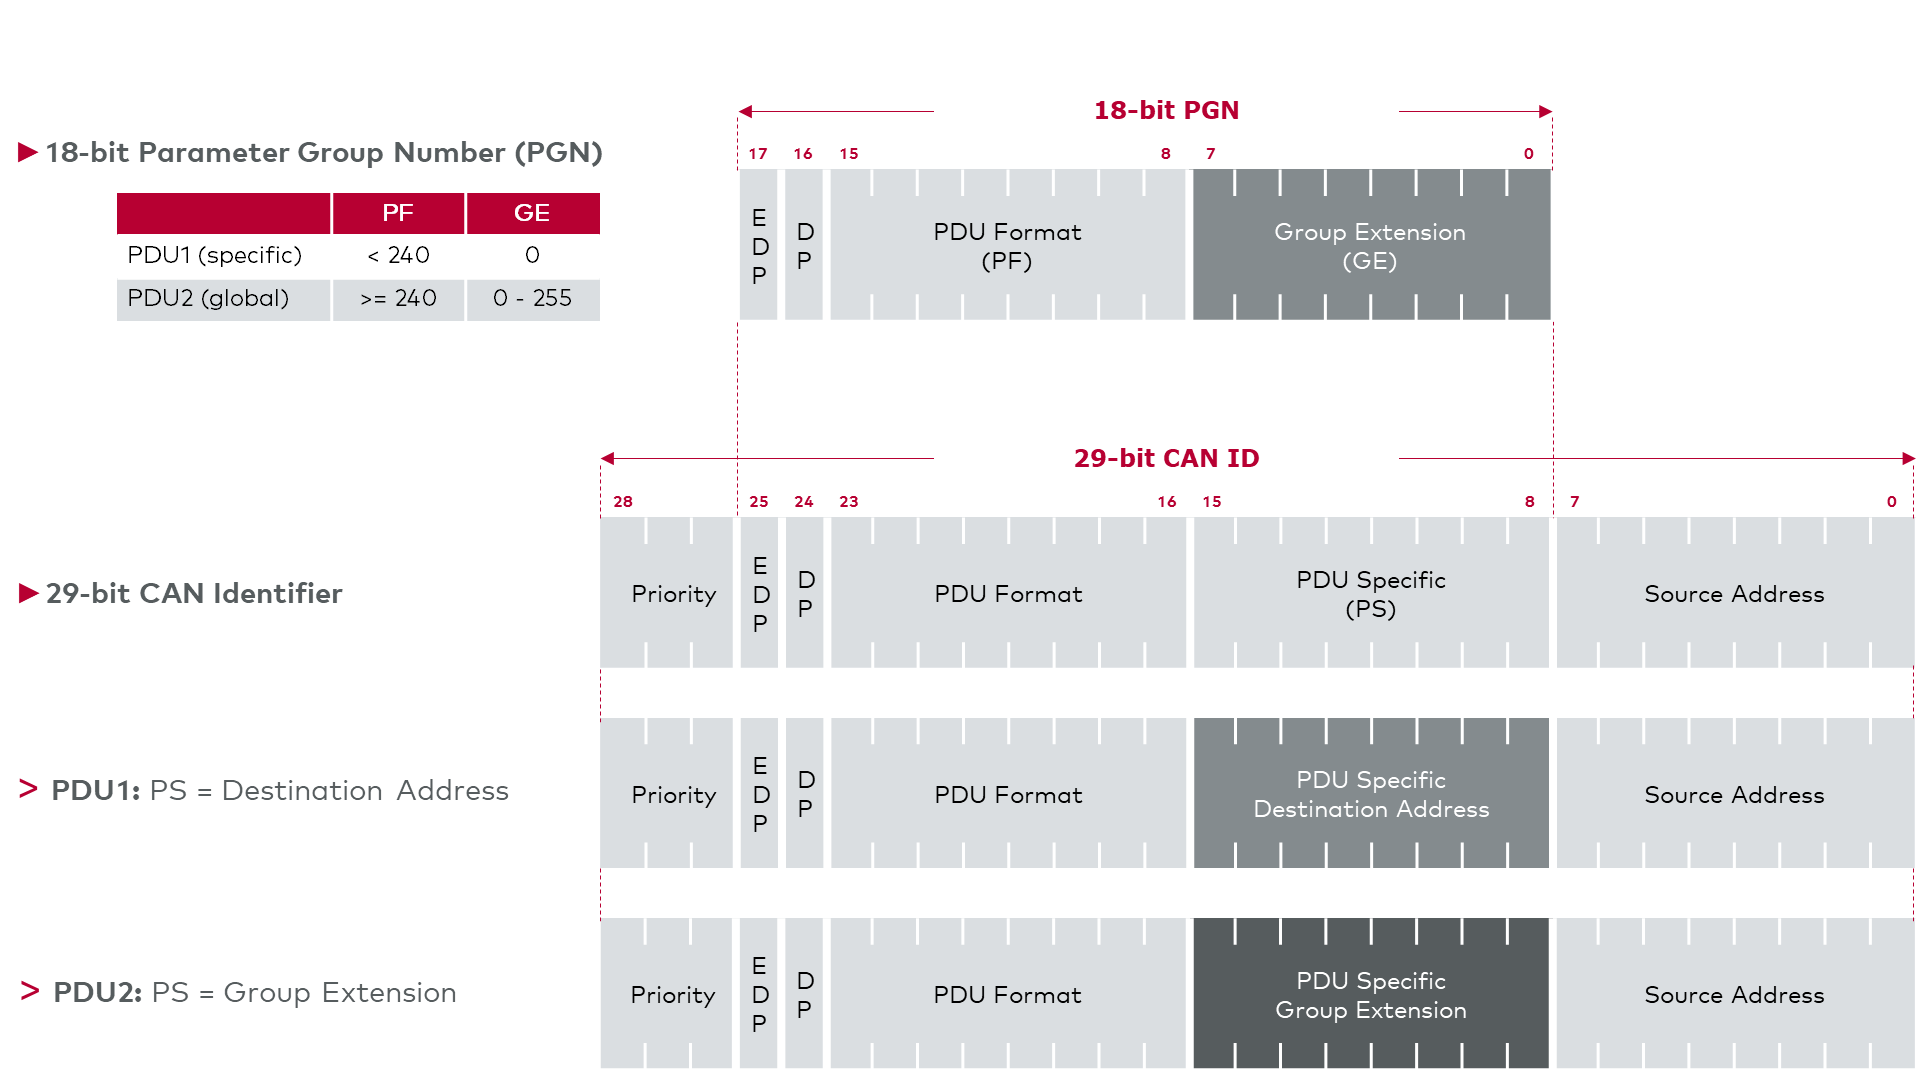
\includegraphics[scale=0.3]{images/j1939header.png}
    \caption{Header einer J1939-Nachricht auf dem CAN-Bus \cite{VektorSAE}(letzter Zugriff: 28.01.2025)}
    \label{fig:j1939header}
\end{figure}
Wie in der Grafik zu sehen, besteht der Header aus einer PGN, einer Quelladresse und einer Priorität. Um nun Nachrichten
an den Motor zu senden, kann eine Nachricht des Gashebels abgefangen werden. Die PGN kann für die eigene Nachricht genutzt
werden. Die Quelladresse kann man auch kopieren. Die Priorität sollte möglichst klein gewählt werden, 
damit die eigene Nachricht bevorzugt wird. In der eigenen Nachricht kann dann die gewünschte Gashebelposition gesendet werden.

\begin{itemize}
    \item Was passiert bei Veränderung der Gashebelposition?
    \item Wie passiert die Rückmeldung
\end{itemize}
Was muss ich dabei beachten?
Muss eine Rückmeldung für die Eingaben geschehen? Wenn ja, wie?
(kleiner OLED-Bildschirm oder App)
